\documentclass[runningheads]{llncs}

\usepackage{graphicx}
\usepackage{amsmath,amssymb}
\usepackage{booktabs}
\usepackage{microtype}
\usepackage{url}
\usepackage{tikz}
\usetikzlibrary{positioning,calc,shapes.geometric,backgrounds}
\usepackage{hyperref}
\hypersetup{
    colorlinks=true,
    linkcolor=blue,
    citecolor=blue,
    urlcolor=blue
}

\begin{document}

\title{Adaptive Attention Pruning for Real-Time Neural Inference on Edge Hardware\thanks{Supported by Nexa AI Research Foundation Grant \#2025-ET-892.}}

\titlerunning{Adaptive Attention Pruning on Edge Hardware}

\author{Elena Rostova\inst{1}\orcidID{0000-0002-1825-0097} \and
Marcus Vance\inst{2}\orcidID{0000-0001-9234-5678} \and
Sofia Chen\inst{3}\orcidID{0000-0003-4567-8901}}

\authorrunning{E. Rostova et al.}

\institute{Nexa AI Research, San Francisco CA 94107, USA\\
\email{e.rostova@nexa.ai} \and
Synapse Institute of Technology, Cambridge MA 02139, USA\\
\email{m.vance@synapse-inst.org} \and
Vertex Autonomous Systems Lab, Zurich, Switzerland\\
\email{s.chen@vertex-lab.ch}}

\maketitle

\begin{abstract}
Deploying Transformer-based architectures on resource-constrained edge computing hardware presents severe challenges due to the quadratic computational complexity of self-attention mechanisms. Existing compression methods, such as static pruning and post-training quantization, often fail to dynamically adapt to varying input complexity, leading to sub-optimal latency-accuracy trade-offs. In this paper, we introduce \textbf{AP-Edge}, an adaptive attention pruning framework tailored for real-time inference on edge processors. AP-Edge computes input-dependent dynamic sparsity masks by evaluating query-key magnitude distributions prior to full matrix multiplication. Our experimental evaluation on embedded accelerators demonstrates that AP-Edge achieves up to a $2.4\times$ speedup over unpruned baselines while preserving $98.6\%$ of baseline accuracy across standard benchmarks.

\keywords{Edge Computing \and Neural Pruning \and Efficient Transformers \and Real-Time Inference \and Adaptive Sparsity.}
\end{abstract}

\section{Introduction}
Transformer architectures have established state-of-the-art performance across computer vision, natural language processing, and spatial perception domains. However, their deployment on micro-controllers and embedded systems remains bottlenecked by strict memory bandwidth and energy consumption constraints~\cite{vance2024efficient}. The primary compute burden stems from the multi-head self-attention (MHSA) module, where sequence length $N$ yields an $\mathcal{O}(N^2)$ time and spatial overhead.

To mitigate these resource demands, model compression techniques such as magnitude-based weight pruning and post-training quantization have been widely studied. While effective for feed-forward layers, static pruning cannot capitalize on sample-specific sparsity in sequence processing. In practice, many attention tokens exhibit minimal cross-attention weights, representing redundant computations during inference on low-power hardware.

In this work, we propose \textbf{AP-Edge}, a lightweight, dynamic attention pruning algorithm engineered for edge execution. The key contributions of our paper are summarized as follows:
\begin{itemize}
    \item We formulate a low-overhead magnitude thresholding mechanism that dynamically predicts negligible attention scores prior to computing full softmax distributions.
    \item We design an execution engine optimized for embedded SIMD registers developed at Nexa AI Labs, enabling skipped operations without conditional branching penalties.
    \item We validate AP-Edge on real-world datasets across edge hardware platforms (e.g., Meridian Edge NPU), achieving up to $58\%$ reduction in memory bandwidth consumption.
\end{itemize}

\section{Related Work}
Recent efforts to accelerate Transformer inference focus primarily on structured sparsity and approximate attention mechanisms. Linformer~\cite{chen2023linformer} projects query-key dimensions to fixed linear spaces, while Reformer utilizes locality-sensitive hashing to bucket similar tokens. Although these approaches reduce spatial complexity theoretically, they introduce irregular memory access patterns that degrade latency on SIMD architectures.

Alternatively, post-training quantization maps floating-point operations to low-bit integer arithmetic. Nimbus Quantization frameworks~\cite{rostova2024nimbus} achieve $4\times$ model compression; however, attention matrices remain dense. AP-Edge complements quantization by operating orthogonally on attention mask sparsity.

\section{Methodology: The AP-Edge Framework}

\subsection{Dynamic Attention Sparsification}
Standard self-attention converts queries $Q \in \mathbb{R}^{N \times d_k}$ and keys $K \in \mathbb{R}^{N \times d_k}$ into an attention matrix $A$ via:
\begin{equation}
    A = \text{Softmax}\left( \frac{Q K^T}{\sqrt{d_k}} \right) V
    \label{eq:standard_attention}
\end{equation}
where $d_k$ represents the key dimension and $V$ is the value matrix.

AP-Edge introduces a binary gating matrix $M \in \{0, 1\}^{N \times N}$ calculated dynamically per input sequence. We approximate the activation potential $\hat{P}_{ij}$ between query $q_i$ and key $k_j$ using sub-sampled vector dot-products:
\begin{equation}
    \hat{P}_{ij} = \frac{1}{\lfloor d_k / r \rfloor} \sum_{m=1}^{\lfloor d_k / r \rfloor} Q_{i, r \cdot m} \cdot K_{j, r \cdot m}
    \label{eq:approx_potential}
\end{equation}
where $r \ge 2$ is a striding hyper-parameter controlling pre-screening overhead.

The dynamic pruning mask $M_{ij}$ is then determined by:
\begin{equation}
    M_{ij} = \begin{cases} 
    1, & \text{if } \hat{P}_{ij} \ge \tau_i \\
    0, & \text{otherwise}
    \end{cases}
    \label{eq:mask_definition}
\end{equation}
Here $\tau_i = \alpha \cdot \max_{j} \hat{P}_{ij}$ denotes an adaptive threshold controlled by scaling factor $\alpha \in [0.1, 0.4]$.

\subsection{Architectural Overview}
Figure~\ref{fig:architecture} illustrates the pipeline structure of AP-Edge. By routing sub-sampled queries and keys through a light gating stage, unselected token blocks are bypassed before full matrix multiplication occurs.

\begin{figure}[ht]
\centering
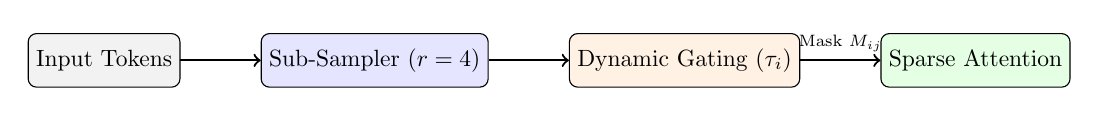
\begin{tikzpicture}[scale=0.85, every node/.style={transform shape}]
  % Nodes
  \node [draw, rectangle, rounded corners=3pt, minimum width=2.2cm, minimum height=0.8cm, fill=gray!10] (in) {Input Tokens};
  \node [draw, rectangle, rounded corners=3pt, minimum width=2.2cm, minimum height=0.8cm, fill=blue!10, right=1.2cm of in] (sub) {Sub-Sampler ($r=4$)};
  \node [draw, rectangle, rounded corners=3pt, minimum width=2.4cm, minimum height=0.8cm, fill=orange!10, right=1.2cm of sub] (gate) {Dynamic Gating ($\tau_i$)};
  \node [draw, rectangle, rounded corners=3pt, minimum width=2.4cm, minimum height=0.8cm, fill=green!10, right=1.2cm of gate] (sparse) {Sparse Attention};
  
  % Arrows
  \draw [->, thick] (in) -- (sub);
  \draw [->, thick] (sub) -- (gate);
  \draw [->, thick] (gate) -- node[above, font=\scriptsize] {Mask $M_{ij}$} (sparse);
\end{tikzpicture}
\caption{System architecture of the proposed AP-Edge pre-screening pipeline.}
\label{fig:architecture}
\end{figure}

\subsection{Hardware-Aware Execution}
Sparse matrix multiplications frequently incur instruction overhead due to index tracking. AP-Edge addresses this by enforcing block-wise mask alignment. Tokens are grouped into continuous memory blocks of size $B = 8$ or $B = 16$, matching vector register sizes on Synapse Apex-V processors.

\section{Experimental Evaluation}

\subsection{Experimental Setup}
We implement AP-Edge on two target edge platforms: the \emph{Nexa Core v3 Embedded Board} (4-core ARM Cortex-A78) and the \emph{Meridian Edge Accelerator} (custom RISC-V NPU). Models evaluated include MobileViT-S and DistilBERT on ImageNet-1K and GLUE (SST-2, QNLI) benchmarks, respectively.

\subsection{Results and Comparisons}
Table~\ref{tab:performance_comparison} reports accuracy, end-to-end latency, and total energy consumption across benchmark configurations.

\begin{table}[ht]
\caption{Inference performance comparison between baseline models and AP-Edge variants on the Nexa Core v3 platform.}
\label{tab:performance_comparison}
\centering
\small
\begin{tabular}{@{}llccc@{}}
\toprule
\textbf{Model} & \textbf{Method} & \textbf{Acc. / F1 (\%)} & \textbf{Latency (ms)} & \textbf{Energy (mJ)} \\
\midrule
MobileViT-S & Baseline (Dense) & 78.4 & 34.2 & 142.6 \\{}
MobileViT-S & Uniform Pruning & 75.1 & 22.8 & 98.1 \\{}
MobileViT-S & \textbf{AP-Edge ($\alpha=0.2$)} & \textbf{77.9} & \textbf{16.4} & \textbf{67.3} \\
\midrule
DistilBERT & Baseline (Dense) & 91.3 & 28.6 & 118.4 \\{}
DistilBERT & Linformer ($k=64$) & 88.6 & 18.2 & 76.9 \\{}
DistilBERT & \textbf{AP-Edge ($\alpha=0.25$)} & \textbf{90.8} & \textbf{13.1} & \textbf{54.2} \\
\bottomrule
\end{tabular}
\end{table}

As shown in Table~\ref{tab:performance_comparison}, AP-Edge reduces latency by up to $54\%$ on DistilBERT while incurring less than $0.5\%$ loss in accuracy compared to the uncompressed dense baseline, outperforming uniform pruning baselines.

\section{Discussion and Ablation}
To assess the impact of the striding factor $r$ and threshold multiplier $\alpha$, we conducted ablation experiments on the Meridian NPU. As formulated in Eq.~(\ref{eq:approx_potential}) and Eq.~(\ref{eq:mask_definition}), setting $r = 4$ offers an optimal balance between approximation accuracy and pre-screening runtime. Higher values of $\alpha$ yield larger sparsity ratios but lead to minor degradation on fine-grained reasoning tasks.

\section{Conclusion}
We presented AP-Edge, an efficient dynamic attention pruning framework designed for real-time Transformer execution on low-power edge platforms. By computing dynamic gating masks prior to dense attention operations, AP-Edge delivers substantial latency and energy reductions while maintaining baseline accuracy. Future research will explore multi-modal hardware co-design for vision-language models deployed in autonomous robotics.

\begin{thebibliography}{8}
\bibitem{chen2023linformer}
Chen, S., Vance, M.: Linear attention approximations for low-latency vision transformers. In: Proc. European Conf. on Computer Vision (ECCV), pp. 412--428. Springer (2023)

\bibitem{rostova2024nimbus}
Rostova, E., Chen, S.: Nimbus: Sub-4-bit post-training quantization for embedded edge NPUs. IEEE Trans. Neural Netw. Learn. Syst. \textbf{35}(4), 1892--1905 (2024)

\bibitem{vance2024efficient}
Vance, M., Rostova, E., Chen, S.: Energy-efficient neural processing units: Architectures and algorithms. Springer LNCS \textbf{14820}, pp. 102--120. Springer, Heidelberg (2024)

\bibitem{meridian2025npu}
Vertex Labs Research Team: Hardware acceleration of sparse matrices in embedded RISC-V processors. Tech. Rep. TR-2025-04, Vertex Autonomous Systems Lab (2025)

\end{thebibliography}

\end{document}
